%% (c) 2016 OPITZ CONSULTING GmbH Thomas Papendieck
\documentclass{beamer}


\usetheme{Montpellier}
%\usetheme{Madrid}
%\usepackage{ngerman}

\usepackage[utf8]{inputenc}
\usepackage[german]{babel}
\usepackage{tikz}
\usetikzlibrary{calc}
\usepackage[T1]{fontenc}
\usepackage{subfiles}
\usepackage{graphicx}
\usepackage{textcomp}
\usepackage{listings}
\usepackage{datetime}
\usepackage[scaled]{beramono}
\usepackage{helvet}
\usepackage{amssymb}
\renewcommand{\familydefault}{\sfdefault}
\usefonttheme{professionalfonts} % using non standard fonts for beamer
%\usefonttheme{serif} % default family is serif
%\definecolor{bulgarianrose}{rgb}{0.28, 0.02, 0.03}
%\definecolor{byzantium}{rgb}{0.44, 0.16, 0.39}
\usepackage{color}
%\usepackage[pdfborder={0 0 0},colorlinks=false]{hyperref}
\lstloadlanguages{Java}
\lstset{numbers=left
 , numberstyle=\tiny
 , language=Java
 , numbersep=5pt
 , identifierstyle=\color{black}
 , keywordstyle=\color{blue}
 , stringstyle=\color{red}
 , commentstyle=\color{green}
 , basicstyle=\footnotesize\ttfamily
 , classoffset=0
 , morekeywords={true,false}
 , keywordstyle=\color{byzantium}\bfseries
 , classoffset=1
 , morekeywords={String,int}
 , keywordstyle=\color{blue}\bfseries
 , classoffset=0
 , frame=tRBl
}
\definecolor{coolblack}{rgb}{0.0, 0.18, 0.39}
\setbeamersize{text margin left=15pt,text margin right=20pt}
\setlength{\rightmargin}{30pt}
\setbeamertemplate{itemize items}{\color{coolblack}{$\blacksquare$}}

\setbeamercolor{frametitle}{fg=coolblack}
\setbeamercolor{section in toc}{fg=coolblack}
\setbeamertemplate{navigation symbols}{}
\setbeamertemplate{background canvas}{%
\begin{tikzpicture}
    \clip (0,0) rectangle (\paperwidth,\paperheight);
	\draw[gray,thin] (0.3,0.3) rectangle (\paperwidth-8,\paperheight-8);
\end{tikzpicture}}

\useoutertheme{infolines}


\beamersetuncovermixins{\opaqueness<1>{25}}{\opaqueness<2->{15}}
\setbeamertemplate{footline}
{
  \leavevmode%
   \hspace{37pt}\color{gray}{\makebox[.915\linewidth]{\rule{.95\linewidth}{0.1pt}}}
  \hbox{%
  \begin{beamercolorbox}[ht=2.25ex,left]{author in head/foot}%
  \setlength\fboxrule{0pt}%
  \hspace{8pt}\fbox{
\includegraphics[height=.6cm]{opitz-consulting-logo}}  %
\color{gray}{\tiny\today \hfill%
 \insertshorttitle\hfill%
    \textcopyright OPITZ CONSULTING GmbH  \hfill \insertframenumber{} / \inserttotalframenumber}%\hfill
  \end{beamercolorbox}
}%
  \vskip3ex%
}{}


\newcommand{\whitepause}{\addtocounter{beamerpauses}{-1}\pause\color<+>{white}}

\begin{document}
\title{Software Quality with JUnit and Mockito}  
\author{Thomas Papendieck}
\date{\today} 

\begin{frame}%[plain]
\tikz[overlay, remember picture] {
  \coordinate (picture) at ($(current page.north west)+(13pt, -7pt)$);
  \node [below right] at (picture) {
\includegraphics[height=.8cm]{opitz-consulting-logo}};
}% <-- Das ist wichtig!
\tikz[overlay, remember picture] {
  \coordinate (picture) at ($(current page.north west)+(\linewidth-120pt, -90pt)$);
  \node [below right] at (picture) {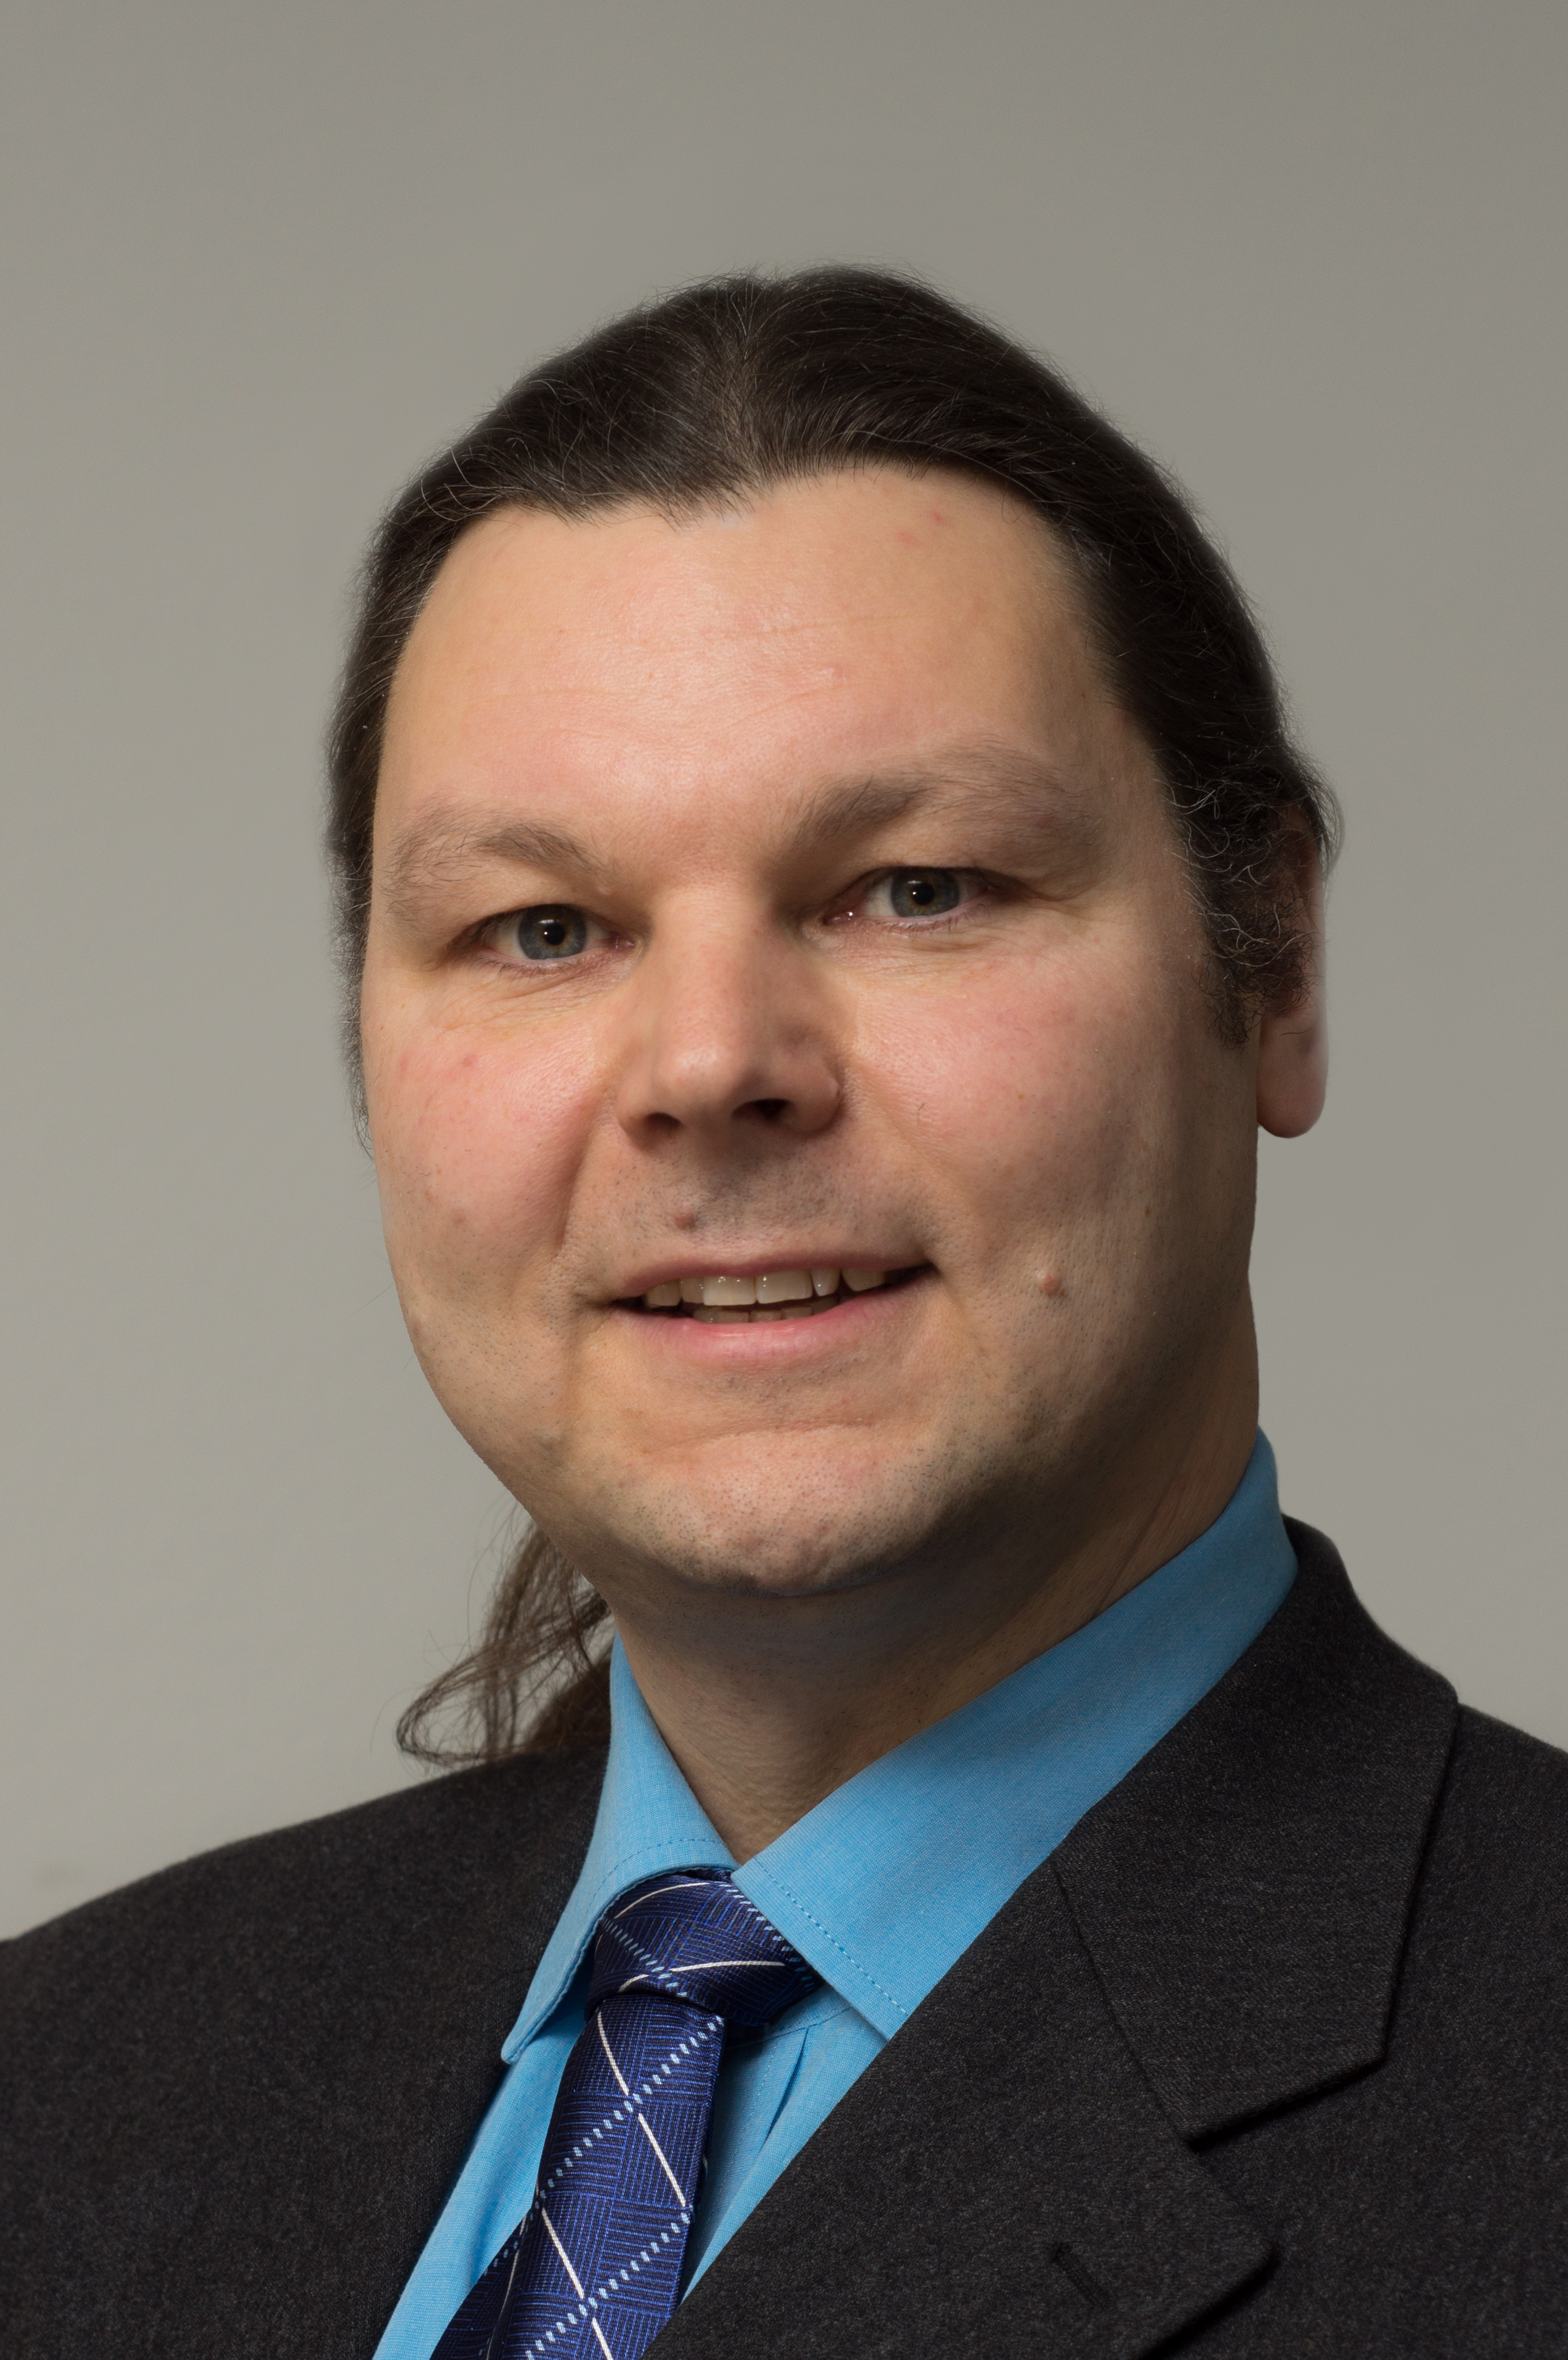
\includegraphics[height=3cm]{OC-Mitarbeiter-tpd}};
}% <-- Das ist wichtig!
\tikz[overlay, remember picture] {
  \coordinate (picture) at ($(current page.north west)+(4pt, -33pt)$);%
   \node [below right] at (picture) {\hspace{1px}\colorbox{gray}{\vspace{3em}
   \hspace{.975\textwidth }
  }}%
}% <-- Das ist wichtig!
\tikz[overlay, remember picture] {
  \coordinate (picture) at ($(current page.north west)+(\linewidth-70pt, -20pt)$);
  \node [below right] at (picture) {
\includegraphics[height=25px]{FrontPageLogo}};
}% <-- Das ist wichtig!
\tikz[overlay, remember picture] {
  \coordinate (picture) at ($(current page.north west)+(4pt, -46pt)$);%
   \node [below right] at (picture) {%
   \Large \textbf{\color{coolblack}{ \inserttitle   }}%
   }%
}% <-- Das ist wichtig!
\tikz[overlay, remember picture] {
\coordinate (picture) at ($(current page.north west)+(4pt, -28pt)$);%
 %   \clip (0,0) rectangle (\paperwidth,\paperheight);
	\draw[gray,thin] (0,-.500) -- (\textwidth,-0.5);
}% <-- Das ist wichtig!
\setlength\fboxrule{0.4pt}%
\vfill
 
{ \textbf{Thomas Papendieck}\\Senior--Consultant\\\vspace{2em}OPITZ CONSULTING GmbH\vspace{2em}}

{University of applied science\\Fulda}
\end{frame}

\begin{frame}
\frametitle{Agenda}\tableofcontents
\end{frame} 

\subfile{Why_do_we_concern}

\subfile{Requirements_on_UnitTests}
\subfile{Requirements_on_tested_code}
\end{document}